\chapter{Proposed Design and Framework}


\section{System Design}

\begin{figure}[here]
\begin{center}    
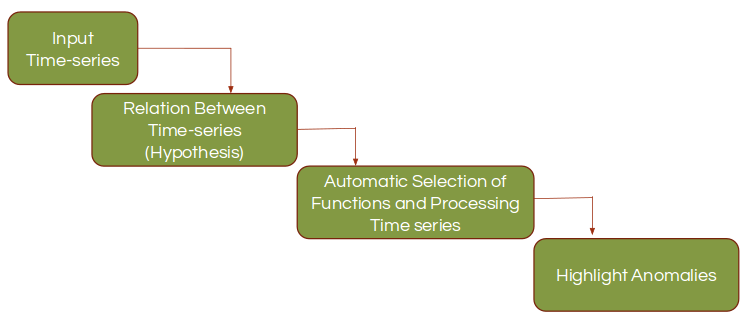
\includegraphics[scale=0.5]{System}
\caption{System Design}
\label{fig:SystemDesign}
\end{center}
\end{figure}


So figure \ref{fig:SystemDesign} explains the overall design of the system and its modules. We have made some assumption regarding system as follows:

\begin{enumerate}

\item Given time series should be of the same time period.
\item Each time series should be present in different file.

\end{enumerate}

\subsection {Input Time-series}

Here, give option to user to input number of time series and accordingly, provide option to select time series in CSV format. Currently, we have thought of keeping restriction that CSV file should contain only one time series. Also, ask user whether he wants to smooth time series or not. Smoothing of time series will be done using Exponential Moving Average technique. $\alpha$  factor for same will be considered as \[ 2 / (1+ period) \].  Where period is considered as up to how much of previous values should have effect on today's value. By default, we have kept it as 14. If user has technical knowledge then option to select period can be provided.

\subsection {Relation Between Time-series (Hypothesis)}

Normal behavior of the time series should be stated somehow, so that we can detect anomaly in the data. So, to get this input from user, we will be providing \textit{n*n} matrix with some default value, where '\textit{n}' corresponds to the number of time series user gave as an input. Now by filling each cell in the matrix, user can specify the relation between any 2 time series as follows:


\begin{itemize}

\item \textbf{1:} Positive Correlation
\item \textbf{-1:} negative Correlation
\item \textbf{0:} Random Relation
\item \textbf{2:} User is not aware but is interested in finding relation, if exist any
\item \textbf{Default:} User is not aware of any relation and also any doesn’t exist according to user

\end{itemize}

If correlation exists, then we may also take input from user maximum lag factor to consider. If not provided any, then by default it will be taken as -15 to +15. We may also ask user, whether to consider only positive lag, negative lag or both types of lag.

\subsection {Automatic Selection of Functions and Processing Time series}

Now, after taking proper input, it is time to execute appropriate function for each of the provided input types.

\subsection {Highlight Anomalies}

After execution, display what tests were performed and what were their results. Detailed values will be provided if asked specifically. Different Graphs/Charts possible with the output can be generated on user demand. Provide an option to user whether he would like to see the results with some different threshold value other than the taken by library. Provide all the functionalities present in the system and ask user, if he wants to run some specific tests on the input time series.

\section{Test Criterion for Hypothesis}

In the last chapter, we stated some hypothesis. Now, here we state what tests can be performed to detect anomalies for each of the hypothesis.

\subsection{Hypothesis 1}

\begin{itemize}

\item Starting with granularity of year-wise, find out cross-correlation, considering various lag factor up to 15,  between arrival and wholesale and check that overall it is positive or negative.

\item Go on decrease the granularity. Next will be season-wise. For a particular season, how arrival and wholesale price are behaving. Point out where, this correlation becomes positive.

\item Similar thing can be done for month-wise as well as fortnight data.

\item Note that, correlation mentioned here is just one of the method. There can be various other methods to define the behavior of 2 time-series.

\item \textbf{Slope Based Detection:} Calculate the slope of both time-series daywise and compare. \textit{Assumption:} Data is smoothed. Since day-wise is taken, if data is not smoothed then it may generate many “spikes”. So if data is not smoothed, then before applying this technique, either apply smoothing or take weekly average. If granularity of data is daywise, then smoothing can help. If data is reported once-twice weekly, then taking average weekly and then calculating slope day-wise may help.

\item \textbf{Linear Regression Based Method:} We can train model using linear regression. Then find out the difference between actual and predicted value for each of the data point and plot a histogram. From these points we can try to find out points which are going very much out of the way using method like MAD test.

\end{itemize}

\subsection{Hypothesis 2}

\begin{itemize}

\item Starting with granularity of year-wise, find out cross-correlation, considering various lag factor up to 15,  between arrival and wholesale and check that overall it is positive or negative.

\item Go on decrease the granularity. Next will be season-wise. For a particular season, how arrival and wholesale price are behaving. Point out where, this correlation becomes positive.

\item Similar thing can be done for month-wise as well as fortnight data.

\item Note that, correlation mentioned here is just one of the method. There can be various other methods to define the behavior of 2 time-series.

\item \textbf{Slope Based Detection:} Calculate the slope of both time-series daywise and compare. \textit{Assumption:} Data is smoothed. Since day-wise is taken, if data is not smoothed then it may generate many “spikes”. So if data is not smoothed, then before applying this technique, either apply smoothing or take weekly average. If granularity of data is daywise, then smoothing can help. If data is reported once-twice weekly, then taking average weekly and then calculating slope day-wise may help.

\item \textbf{Linear Regression Based Method:} We can train model using linear regression. Then find out the difference between actual and predicted value for each of the data point and plot a histogram. From these points we can try to find out points which are going very much out of the way using method like MAD test.

\item Spike Detection methods

\end{itemize}

\subsection{Hypothesis 3}

\begin{itemize}

\item One can use prediction based model like ARIMA \cite{arima} to test this hypothesis. If method mentioned in \cite{arima} is used then there is no need to align time-series into phase, as method mentioned in it take care of it. One can train the model considering some period for 8 years and can be tested on remaining 2 years. Difference in actual and predicted value is seen and one above some threshold value is reported. Also, while generating model, different window size can be considered. If some other technique is used, then one may need to align time series into common phase. That can be done using cross-correlation method, considering lag factor of around 15 days. Lag with the highest correlation value is considered.

\item One can also apply graph based anomaly detection technique as mentioned in \cite{nasa} to find out malicious behavior.

\end{itemize}

\subsection{Hypothesis 4}


Here, we need to combine data of multiple places into one, to find out the combined behavior and then compare it with each of the mandi. One of the technique, to combine multiple series is,

\begin{itemize}

\item For Arrivals: take sum from all Mandis
\item For Wholesale-price: Take average
\item Apart from center, if one wants to combine statewise, then for retail price also, one can take average for retail price

\end{itemize}

Other technique, to combine multiple time series is, subspace based transformation, as mentioned in \cite{phdthesisdc}. Then, to compare behavior of each particular mandi time-series with the aggregated one, techniques mentioned to test hypothesis 1 or 2 can be used.

\textbf{Note (Applicable to Onion Case):} Results returned by H1 and H2, consists of all the time periods where arrival-wholesale price and wholesale price-retail price pairs go out of line. There may be case where, for each time of that year it may be going out of line and might not be anomaly. So, to remove such false positives, we can take intersection of results of H1 and results of H3. Similar thing can be done with H2 also, by taking  intersection of results of H2 and results of H3.


